\documentclass{article}
\usepackage[UTF8]{ctex}
\usepackage{amsmath}
\usepackage{amssymb}
\usepackage{graphicx}
\usepackage{geometry}
\geometry{a4paper, margin=2cm}

\newcommand{\problemname}[1]{\begin{center}\Large\bfseries #1\end{center}}
\usepackage{enumitem}

\begin{document}
\problemname{天花板上的小灯}

虽然小凡刚读到小学六年级，可她已经是一个有五年经验的钢琴高手了唷！上个月，还在全市级别的钢琴比赛中获得一等奖了呢！而今天，正是颁奖典礼的好日子 $\cdots\cdots$

在礼堂等待典礼开始的时候，觉得有些无聊的小凡发现了一个有意思的小问题：

在这个礼堂的天花板上，以矩形阵列的形式装着好多好多照明用的小灯，如下图所示：

\begin{center}
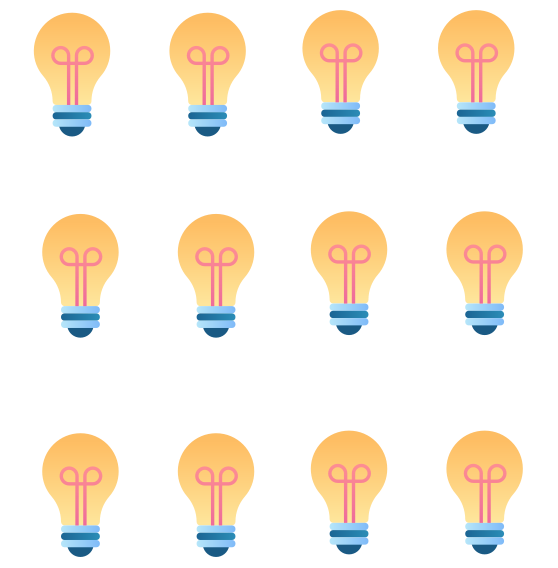
\includegraphics[width=0.7\textwidth]{suanfa35927-7d0473d6f8f9f7e8b385.png}
\end{center}

反正典礼也没开始，我们就和小凡一起数数整个天花板上的小灯一共有多少个吧——当然，只需数下总行数和总列数就可以了。

\subsection*{输入格式}
输入两个用空格分开的整数 $a$、$b$，表示这些小灯的总行数和总列数。保证 $1\lea\le100000$、$1\leb\le100000$。

\subsection*{输出格式}
输出一个整数，表示小灯的总数。

\subsection*{样例输入}
\begin{verbatim}
3 6
\end{verbatim}

\subsection*{样例输出}
\begin{verbatim}
18
\end{verbatim}


\end{document}
